%\documentclass[english, times, mirror]{revdetua}
% use this if you're writing in portuguese:
\documentclass[portuguese, times, mirror]{revdetua}

\usepackage[utf8]{inputenc}
\usepackage{graphicx}
\usepackage{hyperref}

\usepackage{amsmath}
\usepackage{mathtools}

\usepackage{caption}
\usepackage{listings}
\usepackage{color}

\definecolor{dkgreen}{rgb}{0,0.6,0}
\definecolor{gray}{rgb}{0.5,0.5,0.5}
\definecolor{mauve}{rgb}{0.58,0,0.82}

\lstset{frame=tb,
  language=Java,    
  aboveskip=3mm,
  belowskip=3mm,
  showstringspaces=false,
  columns=flexible,
  basicstyle={\small\ttfamily},
  numbers=none,
  numberstyle=\tiny\color{gray},
  keywordstyle=\color{blue},
  commentstyle=\color{dkgreen},
  stringstyle=\color{mauve},
  breaklines=true,
  breakatwhitespace=true,
  tabsize=3
}

\usepackage{tikz}
\usepackage{pgfplots}

% correct bad hyphenation here
\hyphenation{op-tical net-works semi-conduc-tor}

\begin{document}

\Header{1}{4}{Outubro}{2016}{1}
% Note: the month must be in Portuguese

\title{Visão por Computador 2016-17, Guia Prático N.º 5}
\author{Rui Oliveira, Tomás Rodrigues\\ DETI, Universidade de Aveiro \\ Aveiro, Portugal \\ \{ruipedrooliveira, tomasrodrigues\}@ua.pt}
% you should be able to use the \and keyword, but the deti format doesn't like it, for some reason
\maketitle

\begin{resumo}


Pretende-se através deste relatório expor sob forma escrita, o nosso desempenho e objetivos alcançados na aula prática n.5 da unidade curricular de Visão por Computador do Mestrado Integrado de Engenharia de Computadores e Telemática.

Neste relatório pretenderemos explicar as soluções por nós encontradas para a resolução dos diferentes problemas propostos.


\end{resumo} 

\begin{palavraschave} %
visão, computador, imagem digital, opencv, c++, 
 \end{palavraschave} %




\section{Repositório: código fonte}


Todas as soluções dos problemas propostos estão disponível através do seguinte repositório (gitHub) criado para o efeito. \\

\href{http://github.com/toomyy94/CV1617-68779-68129}{http://github.com/toomyy94/CV1617-68779-68129}
\\


A resolução dos problemas do presente guia encontram-se na pasta aula5. Para a resolução dos diferentes exercícios foi usado o \texttt{Code::Blocks IDE}. 



\section{Problemas propostos}



\subsection{Problema \#1 - \textit{Chessboard calibration}}

\subsubsection{Enunciado}
\textit{Compile and test the file \texttt{chessboard.cpp}. This code detects corners in a chessboard pattern using openCV functions and shows the results of the detection for a series of images. Use the available code to calibrate the camera used in the provided images (\texttt{left01.jpg} to \texttt{left13.jpg}). You need to use the function \texttt{calibrateCamera}.}


\subsubsection{Resolução e principais conclusões}

Inicialmente, para a compilação deste exercício foi necessário a linkar a seguinte biblioteca: \texttt{libopencv\_calib3d.so}

Para a calibração da câmara foi usada a seguinte função: 

\begin{lstlisting}[caption=Função calibrateCamera,label=code:C]
calibrateCamera(object_points, image_points, image.size(), intrinsic, distCoeffs, rvecs, tvecs);
\end{lstlisting}

Também para este exercício foram adicionados alguns prints de modo a que seja possível observar o valor das variáveis intrinsics, distortion, translations e rotations.

Por fim, este exercício permite ainda gerar um ficheiro XML com os valores de intrinsics e distortion. 

\begin{lstlisting}[caption=Guardar intrinsics e distortion em XML,label=code:C]
cv::FileStorage fs("../CamParams.xml", cv::FileStorage::WRITE);
fs << "cameraMatrix" << intrinsic << "distCoeffs" << distCoeffs;
fs.release();
\end{lstlisting}


\begin{figure}[ht!]
\centering
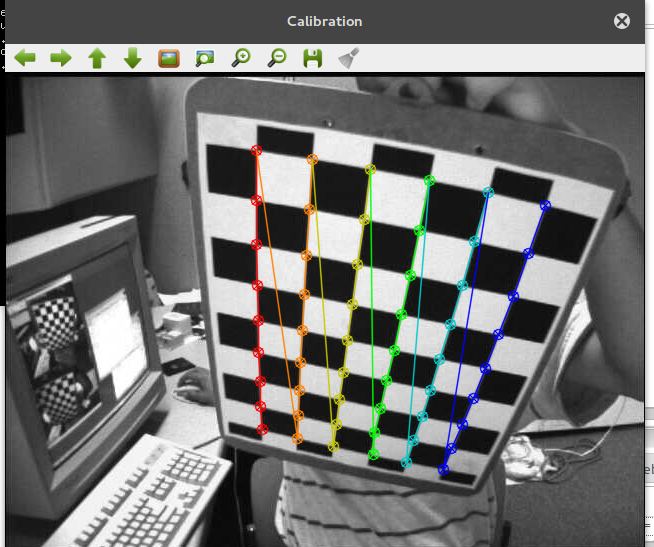
\includegraphics[width=70mm]{img/ex2_in.png}
\caption{Resultado obtido após exercicio 1}
\end{figure}



\subsection{Problema \#2 - \textit{Projection of 3D points in the image}}

\subsubsection{Enunciado}
\textit{Use the function \texttt{cvProjectPoints2()} to project a line orthogonal (normal) to the chessboard (or a wireframe cube) in the provide images into each of the chessboard images using the rotation and translation vectors from the calibration.}

\subsubsection{Resolução e principais conclusões}


Inicialmente, criámos um vetor do tipo \texttt{Point3f} que permitirá guardar os vértices do cubo. Foi usada a função \texttt{push\_back()} para adicionar cada vértice ao vetor.  


\begin{lstlisting}[caption=Criação do vetor para Proposta de resolução do exercício 5,label=code:C]
std::vector<Point3f> new_object_points;
new_object_points.push_back(Point3f(0.0, 0.0, 0.0)); // vertice0
// ... continue
\end{lstlisting}

Seguidamente, foi utilizada a função \texttt{projectPoints} com o seguinte atributos para a criação de uma projeção do cubo.

\begin{lstlisting}[caption=Criação do vetor para Proposta de resolução do exercício 5,label=code:C]
projectPoints(new_object_points, rvecs.at(i), tvecs.at(i), intrinsic, distCoeffs, projected_points);
\end{lstlisting}
  
Finalmente, com a ajuda da função \texttt{line()} foram criadas as linhas do cubo com a cor amarela.

\begin{lstlisting}[caption=Desenhar linhas do cubo,label=code:C]
line(image, projected_points[0], projected_points[1], Scalar(0, 255, 255), 2, 8);
line(image, projected_points[0], projected_points[2], Scalar(0, 255, 255), 2, 8);
// ... continue
\end{lstlisting}


As duas figuras seguinte ilustram o resultado do exercício 2.

\begin{figure}[ht!]
\centering
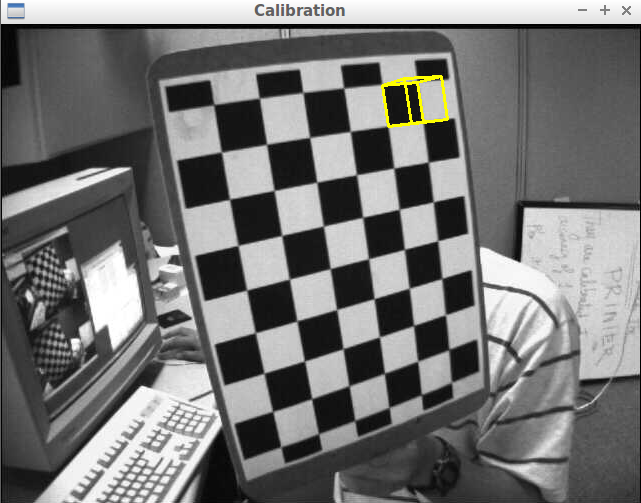
\includegraphics[width=70mm]{img/ex2_r.png}
\caption{Resultado obtido após exercício 2}
\end{figure}

\begin{figure}[ht!]
\centering
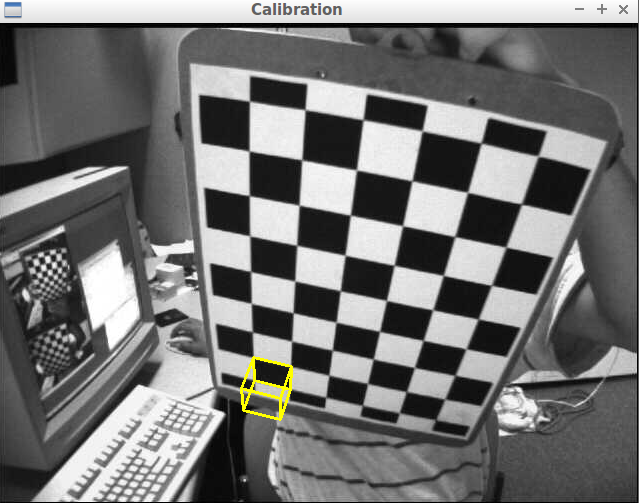
\includegraphics[width=70mm]{img/ex2_r2.png}
\caption{Resultado obtido após exercício 2}
\end{figure}

%%%%%%%%%%%%%%%%%%%%%%%%%%%%%%%%%


\subsection{Problema \#3 - \textit{Using camera on computer}}

\subsubsection{Enunciado}
\textit{Modify the code to use the camera from your computer to process the chessboard (comment the code for reading the provided images to allow switching between camera and provided images). Calibrate you camera with several chessboard images (use \texttt{cvWaitKey()} to move the chessboard position and a pre-defined number of images, for example 10). Be careful to check if the available chessboard is
similar to the one in the provided images. If not, modify the code accordingly. If you want real metric distances, you need to update the code with the real distances of the used chessboard. Save the calibration parameters to a file.}

\subsubsection{Resolução e principais conclusões}


Este exercício permitirá receber imagem proveniente da câmara. Para tal, foi usada a classe \texttt{VideoCapture}. 

Sempre que o utilizador pressiona a tecla \textit{space}, um nova imagem é guardada. Quando são gravadas 13 imagens, o utilizador poderá ver a projeção resultantes, com o desenho do cubo tal como no exercício anterior. 

As duas imagens seguinte, representam a receção da imagens proveniente da câmara. 

\begin{figure}[ht!]
\centering
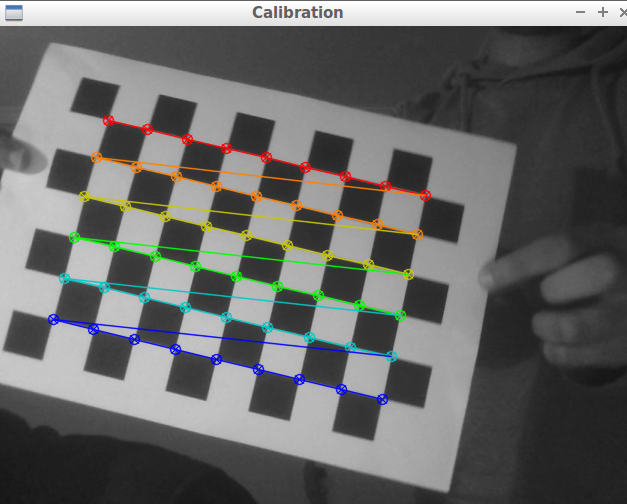
\includegraphics[width=70mm]{img/ex3_in.png}
\caption{Resultado obtido após exercício 3}
\end{figure}

\begin{figure}[ht!]
\centering
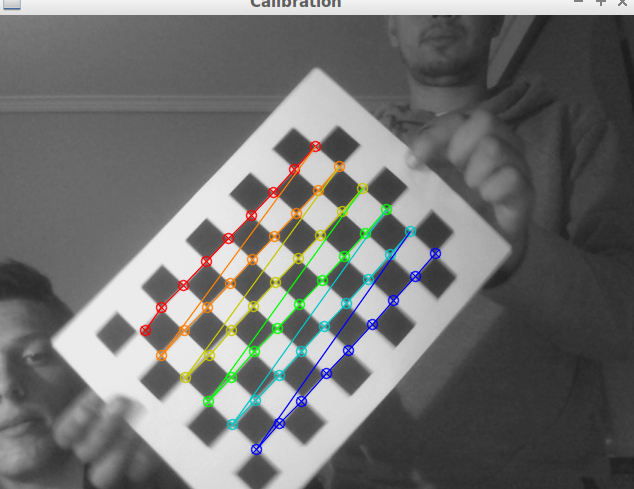
\includegraphics[width=60mm]{img/ex3_in2.png}
\caption{Resultado obtido após exercício 3}
\end{figure}

\newpage
A imagem seguinte, representa a projetação do cubo. 

\begin{figure}[ht!]
\centering
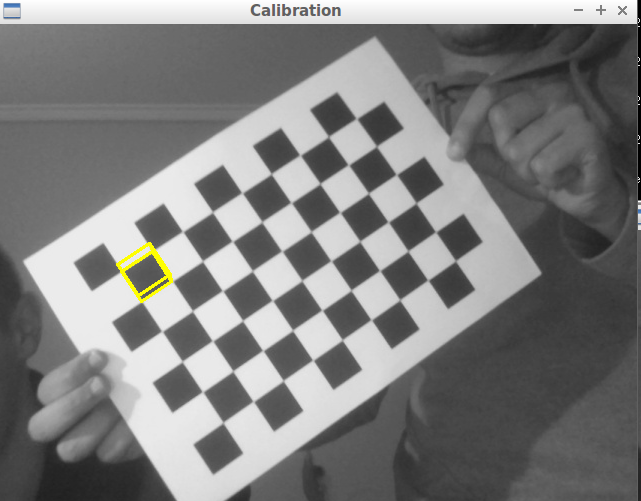
\includegraphics[width=70mm]{img/ex3_r.png}
\caption{Resultado obtido após exercício 3}
\end{figure}


%%%%%%%%%%%%%%%%%%%%%%%%%%%%%%%%%


\subsection{Problema \#4 - \textit{External calibration}}

\subsubsection{Enunciado}
\textit{Calibrate a camera (using the given images or using your computer camera) and save the camera parameter file with another name.
Modify the previous examples to read the intrinsic and distortion parameters from the file and perform external parameters calibration (using function \texttt{solvePnP} ) for a single image with the calibration pattern.}

\subsubsection{Resolução e principais conclusões}

Neste exercício calibramos a câmara com os parâmetros extrínsecos vindos do ficheiro \texttt{CamParams.xml}

Durante a captura de imagem pela câmara, esta foi convertida para cinzento e posteriormente foi aplicado a função \texttt{findChessboardCorners} de modo a obter os \texttt{corners} resultantantes. 






\begin{lstlisting}[caption=Converter para cinza e calcular corners,label=code:C]
cvtColor(image,image,CV_BGR2GRAY);
findChessboardCorners(image, board_sz, corners,0);
\end{lstlisting}



\begin{lstlisting}[caption=Leitura do XML,label=code:C]
cv::Mat intrinsic_matrix;
cv::Mat distortion_coeffs;
cv::FileStorage fs("../CamParams.xml", cv::FileStorage::READ);
if (!fs.isOpened()){
    std::cerr << "Failed to open " << std::endl;
    return 1;
}
fs["cameraMatrix"] >> intrinsic_matrix;
fs["distCoeffs"] >> distortion_coeffs;
fs.release();
\end{lstlisting}

A sequência seguida para a resolução deste exercício foi a seguinte: 

\begin{itemize}
    \item Conversão da imagem obtida pela câmara para \texttt{CV\_BGR2GRAY}
    \item Utilizar o método \texttt{findChessboardCorners()} para detetar os corners
    \item Utilização do método \texttt{solvePnP()}
    \item Utilização do método \texttt{projectPoints()}
    \item Desenhar linhas do cubo 
\end{itemize}


O resultado obtida do exercício 4 encontra-se representado na figura seguinte. 


\begin{figure}[ht!]
\centering
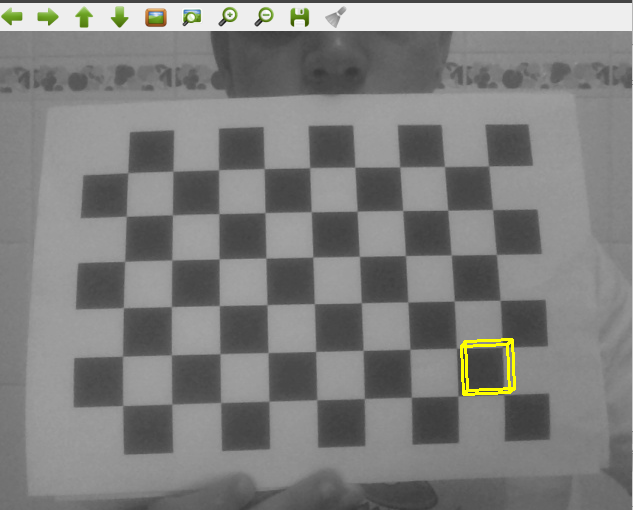
\includegraphics[width=70mm]{img/ex4.png}
\caption{Resultado obtido após exercício 3}
\end{figure}



\begin{thebibliography}{1} % 9



\bibitem{fsound}
Neves, A. J. R.; Dias, P. Slides teóricos Visão por Computador - Aula 5 (2016)


\bibitem{vtk}
OpenCV. \href{hhttp://docs.opencv.org/}{Opencv Documentation}. Web. 15 Outubro 2016. 




\end{thebibliography}

\end{document}
